\documentclass[hide notes]{beamer}
%\documentclass[only notes]{beamer}
\usepackage[english]{babel}
\usepackage{microtype}
\usepackage{environ}
\usepackage{amsmath}
\usepackage[backend=bibtex,style=phys]{biblatex}
\usepackage{doi}
\usepackage{graphicx}
\usepackage{rotating}
\usepackage{tabularx}
\usepackage{dcolumn}
\usepackage{booktabs}
\usepackage{scrextend} % for \footref
\usepackage{hyperref}
\usepackage[nameinlink,capitalize]{cleveref}
\usepackage{siunitx}
\usepackage{floatrow}
\usepackage{bm}
\usepackage{mathtools}

% style stuff
\usetheme{osu}
\hypersetup{hidelinks}
\bibliography{thesis.bib}
% https://latex.org/forum/viewtopic.php?t=25601
\setbeamertemplate{section in toc}{$\bullet$ \inserttocsection}
% https://tex.stackexchange.com/questions/10102/multiple-references-to-the-same-footnote-with-hyperref-support-is-there-a-bett/10116#10116
\crefformat{footnote}{#2\footnotemark[#1]#3}
% http://tex.stackexchange.com/questions/21913/how-can-i-change-the-footnote-line-thickness-length
\renewcommand{\footnoterule}{%
  \kern -3pt
  \hrule width \textwidth height 0.5pt
  \kern 2pt
}
% http://tex.stackexchange.com/questions/21741/how-do-i-change-footnote-font-size-in-beamer-presentation
\let\oldfootnotesize\footnotesize
\renewcommand*{\footnotesize}{\oldfootnotesize\tiny}
% http://tex.stackexchange.com/questions/169745/left-aligning-footnotes-in-beamer
\makeatletter
\renewcommand<>\beamer@framefootnotetext[1]{%
  \global\setbox\beamer@footins\vbox{%
    \hsize\framewidth
    \textwidth\hsize
    \columnwidth\hsize
    \unvbox\beamer@footins
    \reset@font\footnotesize
    \@parboxrestore
    \protected@edef\@currentlabel
         {\csname p@footnote\endcsname\@thefnmark}%
    \color@begingroup
      \uncover#2{\@makefntext{%
        \rule\z@\footnotesep\ignorespaces\parbox[t]{.9\textwidth}{#1\@finalstrut\strutbox}\vskip1sp}}%
    \color@endgroup}%
}
\makeatother

% custom commands
\DeclareMathOperator{\Tanh}{\mathbf{tanh}}
\DeclarePairedDelimiter\ceil{\lceil}{\rceil}
\DeclarePairedDelimiter\floor{\lfloor}{\rfloor}
% footnote without marker
% https://tex.stackexchange.com/questions/30720/footnote-without-a-marker
\newcommand\blfootnote[1]{%
  \begingroup
  \renewcommand\thefootnote{}\footnote{#1}%
  \addtocounter{footnote}{-1}%
  \endgroup
}

% toc slide
\newcommand\tocframe{%
  \frame{\tableofcontents[currentsection,hideallsubsections]}
}
\newcommand\tocframecite[1]{%
  \frame{
    \tableofcontents[currentsection,hideallsubsections]
    \blfootnote{\fullcite{#1}}
  }
}

% use dcolumn
\newcolumntype{d}{D{.}{.}{-1}}
\newcolumntype{e}{D{.}{.}{8}}
\newcolumntype{f}{D{.}{.}{13}}

\title{Essential Reservoir Computing}
%\subtitle{}

\author[Griffith]{Aaron Griffith}
\institute[Ohio State University]{Department of Physics\\Ohio State University}
\date[8/17/2021]{August 17, 2021}

\begin{document}

\begin{frame}[plain]
  \titlepage
\end{frame}

%\setbeamertemplate{footline}[frame number]{\tiny\insertframenumber\,/\,\inserttotalframenumber}
% https://tex.stackexchange.com/questions/434923/frame-number-does-not-work-since-ubuntu-update?noredirect=1&lq=1
\setbeamertemplate{navigation symbols}{\textcolor{osured}{\tiny\insertframenumber\,/\,\inserttotalframenumber}}

\section{Chapter 1: Introduction}

\begin{frame}{What are Reservoir Computers?}
  \begin{columns}
    \column{0.5\textwidth}
    Reservoir computers are an ML tool that learn by example how to...
    \begin{itemize}
    \item transform an input signal into an output signal
    \item infer system state
    \item \textbf{forecast chaotic systems}
      \vspace{1em}
    \item control dynamic systems\footnote[frame]{\fullcite{canaday2020}}
    \end{itemize}
    \vspace{1em}
    In general: they are good at dynamic systems.
    \column{0.5\textwidth}
    \centering
    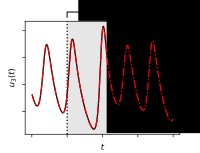
\includegraphics[width=0.95\textwidth]{figures/prediction-example}
  \end{columns}
\end{frame}

\begin{frame}{Compared to other ML Techniques}
  \begin{columns}
    \column{0.6\textwidth}
  Reservoir computers...
  \begin{itemize}
  \item train very quickly via linear regression
  \item do not require much data
  \end{itemize}
  \vspace{2em}
  They are physically interesting:
  \begin{itemize}
  \item naturally handle time-varying signals
  \item use an internal dynamic system to do computation
  \item hardware implementations can use physical systems
  \end{itemize}
  \column{0.4\textwidth}
  \centering
      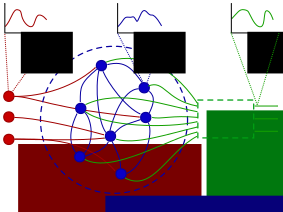
\includegraphics[width=1.0\textwidth]{figures/reservoir}
      \end{columns}
\end{frame}

\begin{frame}{Questions Answered in the next 30 Minutes}
  \begin{itemize}
  \item What is a reservoir computer?
  \end{itemize}
  \vspace{1em}
  {\usebeamercolor[fg]{frametitle}{Contributions:}}
  \begin{itemize}
  \item How simple can I make an RC before it stops working?
  \item What parts of an RC are essential for function?
  \end{itemize}
  \centering
  \begin{columns}
    \column{0.6\textwidth}
    \begin{enumerate}
    \item Introduction
    \item Reservoir Computing
    \item \textbf{Low-Connectivity Reservoirs}
    \item RCs without Reservoirs: NVARs
    \item \textbf{NVARs in Practice}
    \item Conclusion
    \end{enumerate}
    \column{0.4\textwidth}
    \centering
    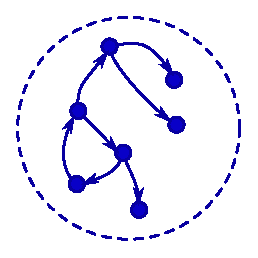
\includegraphics[width=0.6\textwidth]{figures/topology-b}
  \end{columns}
  % needed for... TeX reasons
  %\blfootnote{}
\end{frame}

%\frame{\tableofcontents[hideallsubsections]}

\begin{frame}{Publications}
  \begin{itemize}
  \item {\usebeamercolor[fg]{frametitle}{Chapter 3: Low-Connectivity Reservoirs}} \\
    {\small A.~Griffith, A.~Pomerance, and D.~J.~Gauthier, ``Forecasting chaotic systems with very low connectivity reservoir computers,'' \href{https://doi.org/10.1063/1.5120710}{Chaos \textbf{29}, 123108 (2019)}.}
    \vspace{0.5em}
  \item {\usebeamercolor[fg]{frametitle}{Chapter 5: NVARs in Practice}} \\
    {\small D.~J.~Gauthier, E.~Bollt, A.~Griffith, W.~A.~S.~Barbosa, ``Next generation reservoir computing,'' \href{https://arxiv.org/abs/2106.07688}{(2021), arXiv:2106.07688~[cs.LG]}.}
      \vspace{0.5em}
    \item {\small D.~Canaday, A.~Griffith, and D.~J.~Gauthier, ``Rapid time series prediction with a hardware-based reservoir computer,'' \href{https://doi.org/10.1063/1.5048199}{Chaos \textbf{28}, 123119 (2018)}.}
      \vspace{0.5em}
    \item {\small W.~A.~S.~Barbosa, A.~Griffith, G.~E.~Rowlands, L.~C.~G.~Govia, G.~J.~Ribeill, M.-H.~Nguyen, T.~A.~Ohki, and D.~J.~Gauthier, ``Symmetry-aware reservoir computing,'' \href{https://arxiv.org/abs/2102.00310}{(2021), arXiv:2102.00310~[cs.NE]}.}

  %% \item {\usebeamercolor[fg]{frametitle}{Chapter 3}} \\ \fullcite{griffith2019}
  %% \item {\usebeamercolor[fg]{frametitle}{Chapter 5}} \\ \fullcite{gauthier2021}
  %%   \vspace{1em}
  %% \item \fullcite{canaday2018}
  %% \item \fullcite{barbosa2021}
  \end{itemize}
\end{frame}

\section{Chapter 2: Reservoir Computing}

\tocframe

\begin{frame}{What Is a Reservoir Computer?}
  \begin{itemize}
  \item RC transforms an input signal $\bm{u}(t)$ into an output $\bm{y}(t)$
  \item input $\bm{u}(t)$ acts as driving input to dynamical system $\bm{R}$ \\ (the ``reservoir''),
    $$ \dot{\bm{r}}(t) = \bm{R}(\bm{r}, \bm{u}, t) $$
  \item reservoir response $\bm{r}(t)$ is read-out via $\bm{g}$, and linearly combined into output
    $$ \bm{y}(t) = W_\text{out}\;\bm{g}\left(\bm{r}\left(t\right)\right) $$
  \item read-out $\bm{g}$ models incomplete measurement, is usually identity
  \item reservoir $\bm{R}$ and read-out $\bm{g}$ fixed ahead of time, but $W_\text{out}$ is trained to fit example data
  \end{itemize}
\end{frame}

\subsection{2.3 Echo State Networks}
\begin{frame}{What System to use as Reservoir?}
  \begin{columns}
    \column{0.5\textwidth}
    \begin{itemize}
    \item one common choice: a Echo State Network
    \item network should$^*$ be recurrent\footnote[frame]{\fullcite{jaeger2001}}
    \end{itemize}
    \column{0.5\textwidth}
    \centering
    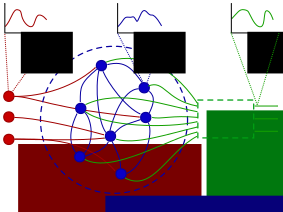
\includegraphics[width=1.0\textwidth]{figures/reservoir}
  \end{columns}
  \begin{align*}
    \dot{\bm{r}}(t) &= - \gamma \bm{r}(t) + \gamma \bm{f}\left( W_r\;\bm{r}(t) + W_\text{in}\;\bm{u}(t) \right) \\
    \bm{y}(t) &= W_\text{out}\;\bm{g}\left(\bm{r}(t)\right)
  \end{align*}
\end{frame}

%\begin{frame}{Reservoir Computer Overview}
%  \centering
%  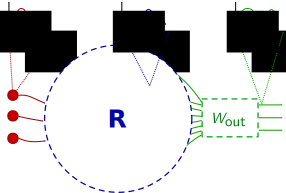
\includegraphics[width=0.8\textwidth]{figures/reservoir-generic}
%\end{frame}

\subsection{2.1 Training an RC}
\begin{frame}{Training an RC}
  % FIXME illustration?
  \begin{itemize}
  \item use example input $\bm{u}_\text{train}(t)$ and example output $\bm{y}_\text{train}(t)$
  \item example input produces example reservoir response $\bm{r}_\text{train}(t)$
  \item Goal: find $W_\text{out}$ such that
    $$ \bm{y}_\text{train}(t) \approx W_\text{out}\;\bm{g}\left(\bm{r}_\text{train}\left(t\right)\right)$$
  \item this is \emph{linear regression}! this is \emph{fast}!
  \item usually, RCs use ridge regression
  \end{itemize}
\end{frame}

\subsection{2.2 Forecasting with an RC}
\begin{frame}{Forecasting with an RC}
  \begin{itemize}
  \item for system forecasting, find $W_\text{out}$ such that
    $$ \bm{u}_\text{train}(t) \approx W_\text{out}\;\bm{g}\left(\bm{r}_\text{train}\left(t\right)\right)$$
  \item after training, feed output of RC back into itself as input and run autonomously
  \end{itemize}
  \centering
  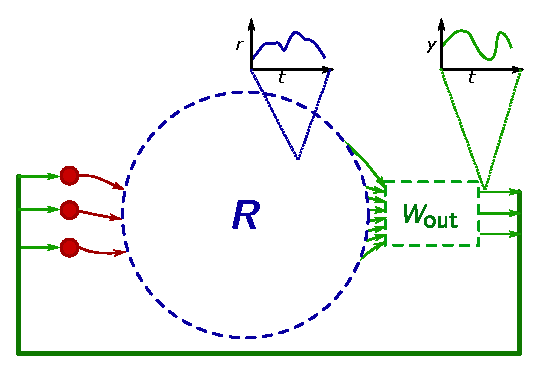
\includegraphics[width=0.6\textwidth]{figures/reservoir-predict}
\end{frame}

\subsection{2.6 Evaluating Reservoirs}
\begin{frame}{Evaluating an RC}
  \begin{columns}
    \column{0.5\textwidth}
    \begin{itemize}
    \item use normalized root-mean-squared error (NRMSE)
    \item for chaotic system forecasting, a forecast \emph{must} diverge eventually, so only calculate for 1 Lyapunov period ($\epsilon_1$)
    \end{itemize}
    \column{0.5\textwidth}
    \centering
    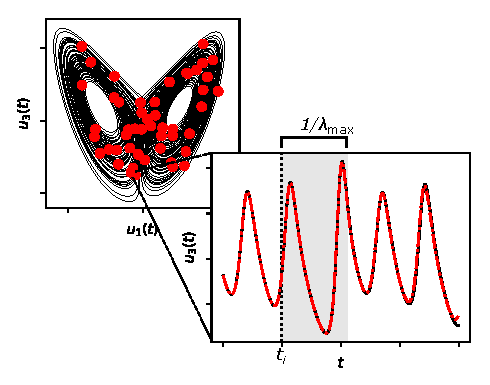
\includegraphics[width=1.0\textwidth]{figures/nrmse-avg}
  \end{columns}
  \vspace{1em}
  \begin{itemize}
  \item $\epsilon_1$ is misleading: if forecasting starts near an unstable part of the input system, small errors are amplified
  \item {\usebeamercolor[fg]{frametitle}{Contribution:}}\footnote{\fullcite{griffith2019}} perform $m$ forecasts and average the errors into $\tilde{\epsilon}$
  \end{itemize}
\end{frame}

\subsection{2.4 Constructing ESNs}
\begin{frame}{Constructing ESNs}
  \begin{itemize}
  \item $\gamma$ (node decay rate) is tuned to match input timescale
  \item $f$ (activation function) is traditionally $\tanh$
    \vspace{2em}
  \item $W_r$ and $W_\text{in}$ chosen \emph{randomly}
    \begin{itemize}
    \item $k$, recurrent inputs for each node
    \item $\rho_r$, spectral radius of $W_r$
    \item $\sigma$, probability of external input per node
    \item $\rho_\text{in}$, scale of $W_\text{in}$
    \end{itemize}
    \vspace{2em}
  \item this seems arbitrary and complicated...
  \item What reservoirs work well? What ESN parameters work well?
  \item \emph{How much of this is necessary?}
  \end{itemize}
\end{frame}

\section{Chapter 3: Low-Connectivity Reservoirs}

\tocframecite{griffith2019}

\begin{frame}{Exploring ESN Parameters}
    \begin{columns}
      \column{0.5\textwidth}
      \begin{itemize}
      \item to find parameters that work well, I started using Bayesian optimization
      \item looking for ESNs that work well at forecasting Lorenz~'63 system
        \begin{equation*}
          \begin{aligned}
            \dot{x} &= \sigma \left(y - x\right), \\
            \dot{y} &= x \left(\rho - z\right) - y, \\
            \dot{z} &= x\,y - \beta z,
          \end{aligned}
        \end{equation*}
        with $\sigma = 10$, $\rho = 28$, and $\beta = 8/3$.
      \end{itemize}
      \column{0.5\textwidth}
      \centering
      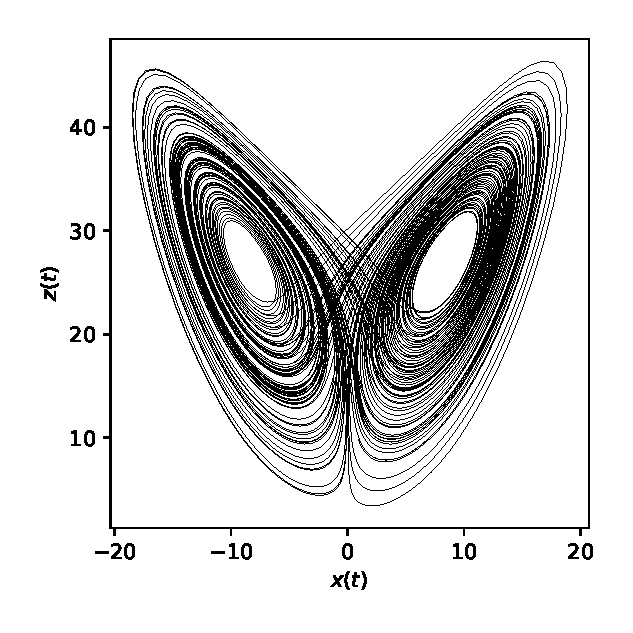
\includegraphics[width=1.0\textwidth]{figures/lorenz}
    \end{columns}
    \blfootnote{\fullcite{lorenz1963}}
\end{frame}

\subsection{3.2 Structure of Low-Connectivity Reservoirs}
\begin{frame}{Surprise!}
  \begin{columns}
    \column{0.6\textwidth}
    \begin{itemize}
    \item while optimizing, a strange result: optimized parameters often had $k = 1$
    \item ESNs with $k = 1$ have very simple structure, but perform as well as $k > 1$
    \item inspired by this, I also look at three other simple structures...
    \end{itemize}
    \column{0.4\textwidth}
    \centering
    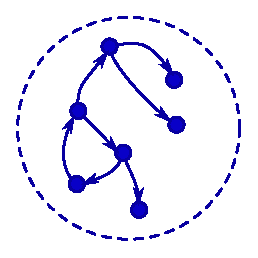
\includegraphics[width=1.0\textwidth]{figures/topology-b}
  \end{columns}
\end{frame}

\begin{frame}{Structure of Low-Connectivity Reservoirs}
  \begin{columns}
      \column{0.4\textwidth}
      \small
      (a) general construction \\
      (b) $k = 1$, single cycle \\
      (c) $k = 1$, cut cycle \\
      (d) \emph{simple cycle reservoir}\footnote[frame]{\fullcite{rodan2011}\label{fn:rodan}} \\
      %(d) \emph{simple cycle reservoir} \\
      (e) \emph{delay line reservoir}\cref{fn:rodan} \\~\\
      %(e) \emph{delay line reservoir} \\~\\
      In all cases, networks with more than one connected component are discarded and regenerated.
      \column{0.6\textwidth}
      \centering
      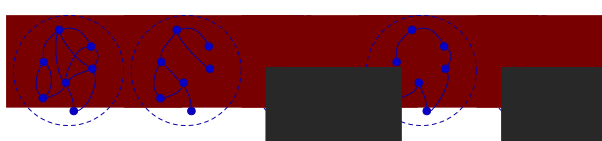
\includegraphics[width=1.0\textwidth]{figures/topology}
  \end{columns}
  %\blfootnote{\fullcite{rodan2011}}
\end{frame}

%% \subsection{3.3 ESN Symmetries and their Consequences}
%% \begin{frame}{Along the Way: ESN~Symmetries~and~their~Consequences}
%%   \begin{itemize}
%%   \item when $f = \tanh$ and $\bm{g}(\bm{r}) = \bm{r}$, ESN forecast equation has $\bm{r} \rightarrow -\bm{r}$ and $\bm{y} \rightarrow -\bm{y}$ symmetry
%%     \begin{align*}
%%       \dot{\bm{r}}(t) &= - \gamma \bm{r}(t) + \gamma \bm{f}\left( W_r\;\bm{r}(t) + W_\text{in}\;W_\text{out}\bm{g}\left(\bm{r}(t)\right)\right) \\
%%       \bm{y}(t) &= W_\text{out}\;\bm{g}\left(\bm{r}(t)\right)
%%     \end{align*}
%%   \item Lorenz does \emph{not}!
%%   \item Solution: break the symmetry by using a non-linear $\bm{g}$\footnote{\fullcite{herteux2020}}
%%     \begin{equation*}
%%       g_i(\bm{r}) = \begin{cases}
%%         r_i & \text{if } i \leq N / 2, \\
%%         r_i^2 & \text{if } i > N / 2.
%%       \end{cases}
%%     \end{equation*}
%%     \end{itemize}
%% \end{frame}

%% \begin{frame}{Example of Symmetric ESN Failure on Lorenz '63}
%%   \centering
%%   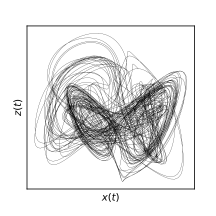
\includegraphics[width=0.7\textwidth]{figures/lorenz-symmetry}
%% \end{frame}

%% \subsection{3.4 Training, Forecasting, and Evaluation}
%% \begin{frame}{Along the Way: $\epsilon_1$ vs. $\tilde{\epsilon}$}
%%   \begin{center}
%%     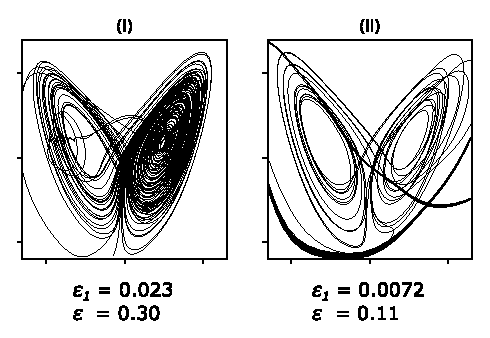
\includegraphics[width=0.7\textwidth]{figures/epsilon-failure}
%%   \end{center}

%%   {\small
%%     (i) overemphasizes lobe where $\epsilon_1$ resides \\
%%     (ii) good short-term forecast, but falls into periodic orbit as $t \rightarrow \infty$}
%% \end{frame}

\subsection{3.5 Results}
\begin{frame}{Results}
  \begin{itemize}
  \item for each structure, I search for the parameters to optimize $\tilde{\epsilon}$ on Lorenz forecasting
  \item in the end, have one ESN from each structure type that performs well
  \item they all perform the same!
  \end{itemize}
  \vspace{2em}
  \centering
  \begin{tabularx}{\linewidth}{l l@{\extracolsep{\fill}} l}
    & Structure & $\tilde{\epsilon}$ \\
    \hline
    (a) & Any $k$ & 0.022 $\pm$ 0.004 \\
    (b) & $k = 1$ with cycle & 0.024 $\pm$ 0.005 \\
    (c) & $k = 1$ no cycle & 0.028 $\pm$ 0.005$^*$ \\
    (d) & cycle & 0.023 $\pm$ 0.008 \\
    (e) & line & 0.024 $\pm$ 0.003$^*$ \\
  \end{tabularx}
  \vspace{3em}
  $^*$ \emph{no recurrence in network!} (against conventional wisdom)
\end{frame}

%% \begin{frame}{Results}
%%   \centering
%%   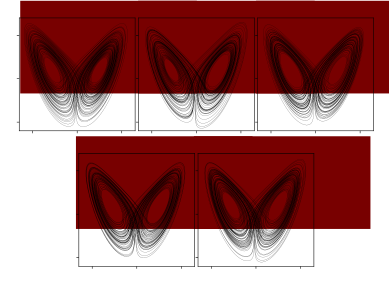
\includegraphics[width=0.7\textwidth]{figures/lowk-attractors}
%% \end{frame}

%% \subsection{3.5.2 ESN Variation}
%% \begin{frame}{ESN Variation}
%%   \begin{itemize}
%%     \item ESN construction is random -- what if I re-generate a network with the same parameters as best performers?
%%   \end{itemize}
%%   \centering
%%   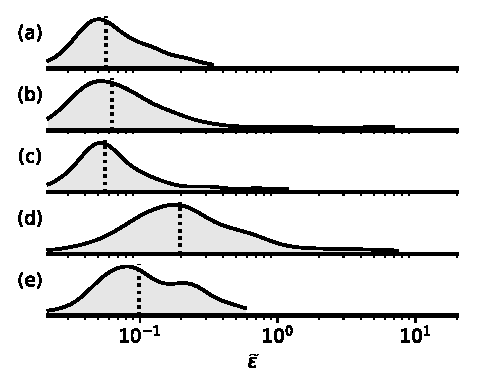
\includegraphics[width=0.7\textwidth]{figures/epsilon-distribution}
%% \end{frame}

\subsection{3.6 Conclusion}
\begin{frame}{Conclusion}
  \begin{itemize}
  \item very simple ESNs can perform as well as ESNs with more complicated connectivity
  \item however, well-performing simple ESNs are harder to find
  \item line networks work well -- so how do line networks behave?
  \end{itemize}
  \begin{center}
    
\includegraphics[width=\textwidth]{figures/line-reservoir}
  \end{center}
  \begin{itemize}
  \item each node has finite rise/fall time, and delays inputs
  \item a line network creates many time-delayed copies of the input and combines them
  \end{itemize}
\end{frame}

\section{Chapter 4: RCs without Reservoirs: NVARs}

\tocframe

\begin{frame}{NVARs are equivalent to ESNs}
  \begin{itemize}
  \item in 2020, Erik Bollt proved that a linear ESN is equivalent to a \emph{vector auto-regression} (VAR)
  \item shortly after, he extended this proof to equivalence between output-nonlinear ESNs ($\bm{g}$ nonlinear) and nonlinear VARs
    \vspace{2em}
  \item a full mathematical equivalence proof that (some) ESNs are exactly equivalent to combining time-delayed copies of the input! \usebeamercolor[fg]{frametitle}{(!!)}
    \blfootnote{\fullcite{bollt2021}}
  \end{itemize}
\end{frame}

\subsection{4.3 Nonlinear Vector Autoregressions (NVARs)}
\begin{frame}{What is a Nonlinear VAR?}
  \begin{itemize}
  \item transforms an input $\bm{u}(t)$ into output $\bm{y}(t)$ via a time-delay vector $\bm{v}(t)$
  \item given a time step $\Delta t$ and tap delays $\tau_0, \dots, \tau_{q-1}$, build
    $$ \bm{v}(t + \Delta t) = \bm{u}(t - \tau_0 \Delta t) \oplus \bm{u}(t - \tau_1 \Delta t) \oplus \cdots \oplus \bm{u}(t - \tau_{q-1} \Delta t) $$
  \item construct the output from a nonlinear function of $\bm{v}$,
    $$ \bm{y}(t + \Delta t) = W_\text{out}\;\bm{g}_\text{n}\left(\bm{v}(t + \Delta t)\right) $$
    \vspace{2em}
    \item note similarity to RC approach: replace $\bm{r}(t)$ with $\bm{v}(t)$, and $\bm{g}(\bm{r})$ with $\bm{g}_\text{n}(\bm{v})$
  \end{itemize}
\end{frame}

\begin{frame}{Nonlinear VAR Overview}
  \centering
  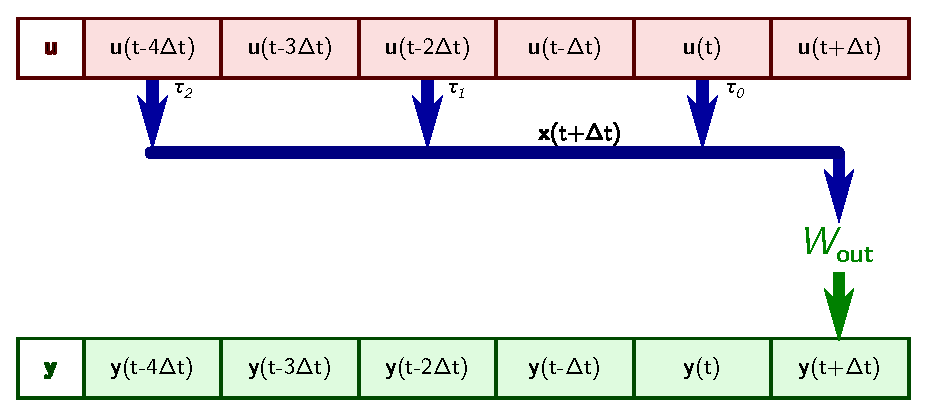
\includegraphics[width=0.9\textwidth]{figures/var-infer}
\end{frame}

\begin{frame}{Training and Testing}
  \begin{itemize}
  \item same process as for RCs!
  \item feed in example input $\bm{u}_\text{train}(t)$ to produce $\bm{v}_\text{train}(t)$, then use ridge regression to find $W_\text{out}$
  \item for forecasting, connect output to input as with RCs, but modify output slightly
    $$ \bm{y}(t + \Delta t) = \bm{u}(t) + W_\text{out}\;\bm{g}_\text{n}\left(\bm{v}(t + \Delta t)\right) $$
  \item testing also uses NRMSE $\epsilon$ and $\tilde{\epsilon}$
  \end{itemize}
\end{frame}

%% \begin{frame}{$\bm{g}$ vs. $\bm{g}_\text{n}$}
%%   \begin{itemize}
%%   \item important: under equivalence, the $\bm{g}$ of the ESN is \emph{not} identical to $\bm{g}_\text{n}$
%%   \item for an ESN with quadratic readout $\bm{g}(\bm{r})$
%%     \begin{equation*}
%%       g_i(\bm{r}) = \begin{cases}
%%         r_i & \text{if } i \leq N, \\
%%         r_{i - N}^2 & \text{if } N < i \leq 2N.
%%       \end{cases}
%%     \end{equation*}
%%   \item equivalent NVAR $\bm{g}_\text{n}(\bm{v})$ has all possible linear and quadratic terms of components of $\bm{v}$
%%     $$ \bm{g}_\text{n}(\bm{v}) = \bm{v} \oplus \ceil{\bm{v} \otimes \bm{v}} $$
%%   \item this suggests an easy extension: keep adding higher order terms to $\bm{g}_\text{n}$ until NVAR works
%%   \end{itemize}
%% \end{frame}

\subsection{4.4 Practical Considerations}
\begin{frame}{Practical Considerations}
  Positives:
  \begin{itemize}
  \item NVARs are equivalent to ESNs, but completely sidestep the issue of choosing a network
  \item replace complicated reservoir with simple time-delay taps
  \item \emph{Why ever use an ESN if an NVAR will work?}
  \end{itemize}
  \vspace{1em}
  Possible problems:
  \begin{itemize}
  \item for $q$ taps, $d$ input dimensions, and $\bm{g}_\text{n}$ with $n$-degree polynomial terms, $W_\text{out}$ has to fit $(qd)^n$ components (expensive!)
  \item mathematically, equivalence only holds for \emph{infinite taps}!
  \item Are NVARs still useful for low $q$ and low $n$?
  \end{itemize}
\end{frame}

\section{Chapter 5: NVARs in Practice}

\tocframecite{gauthier2021}

\begin{frame}{NVARs in Practice}
  To show that NVARs work even in non-theoretical settings, I use them for
  \begin{itemize}
  \item Lorenz '63 state inference
  \item \textbf{Lorenz '63 forecasting}
  \item double-scroll circuit forecasting
  \item Mackey-Glass forecasting
  \end{itemize}
  \vspace{2em}
  I will highlight only Lorenz '63 forecasting -- more details in my dissertation.
\end{frame}

%% \subsection{5.1 State Inference with Lorenz '63}
%% \begin{frame}{Lorenz '63 State Inference}
%%   \begin{itemize}
%%   \item Goal: infer Lorenz $z$ from $x$ and $y$
%%   \item four taps, $\tau_0 = 0$, $\tau_1 = 5$, $\tau_2 = 10$, $\tau_3 = 15$
%%   \item $\Delta t = 0.05$ (20 points per Lyapunov period)
%%   \item $\bm{g}_\text{n}$ includes constant, linear, and quadratic terms
%%     $$ \bm{g}_\text{n}(\bm{v}) = 1 \oplus \bm{v} \oplus \ceil{\bm{v} \otimes \bm{v}} $$
%%   \item Lorenz $z$ has non-zero mean, constant term helps fit that
%%     \vspace{2em}
%%   \item train on 20 time units (400 data points)
%%   \item evaluate on 45 time units (900 data points)
%%   \end{itemize}
%% \end{frame}

%% \begin{frame}{Lorenz '63 State Inference Results}
%%   \begin{center}
%%     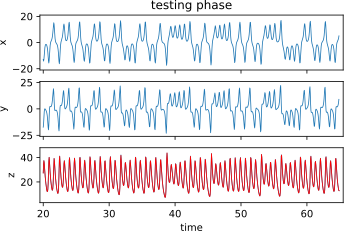
\includegraphics[width=0.8\textwidth]{figures/nvar-infer-lorenz-testing}
%%   \end{center}
%%   \begin{itemize}
%%   \item NRMSE $\epsilon = 1.75\pm0.3\times10^{-2}$
%%   \end{itemize}
%% \end{frame}

\subsection{5.2 Forecasting Lorenz '63}
\begin{frame}{Lorenz '63 Forecasting}
  \begin{itemize}
  \item use two adjacent taps, $\tau_0 = 0$ and $\tau_1 = 1$
  \item $\bm{g}_\text{n}$ includes constant, linear, and quadratic terms of $\bm{v}(t)$
    $$ \bm{g}_\text{n}(\bm{v}) = 1 \oplus \bm{v} \oplus \ceil{\bm{v} \otimes \bm{v}} $$
    \vspace{2em}
  \item NRMSE $\tilde{\epsilon} = 4.51\pm0.85\times10^{-3}$
    (~5$\times$ better than ESN!)
  \item low number of taps, low order nonlinearity
  \end{itemize}
\end{frame}

\begin{frame}{Lorenz '63 Forecasting Results}
  \begin{center}
    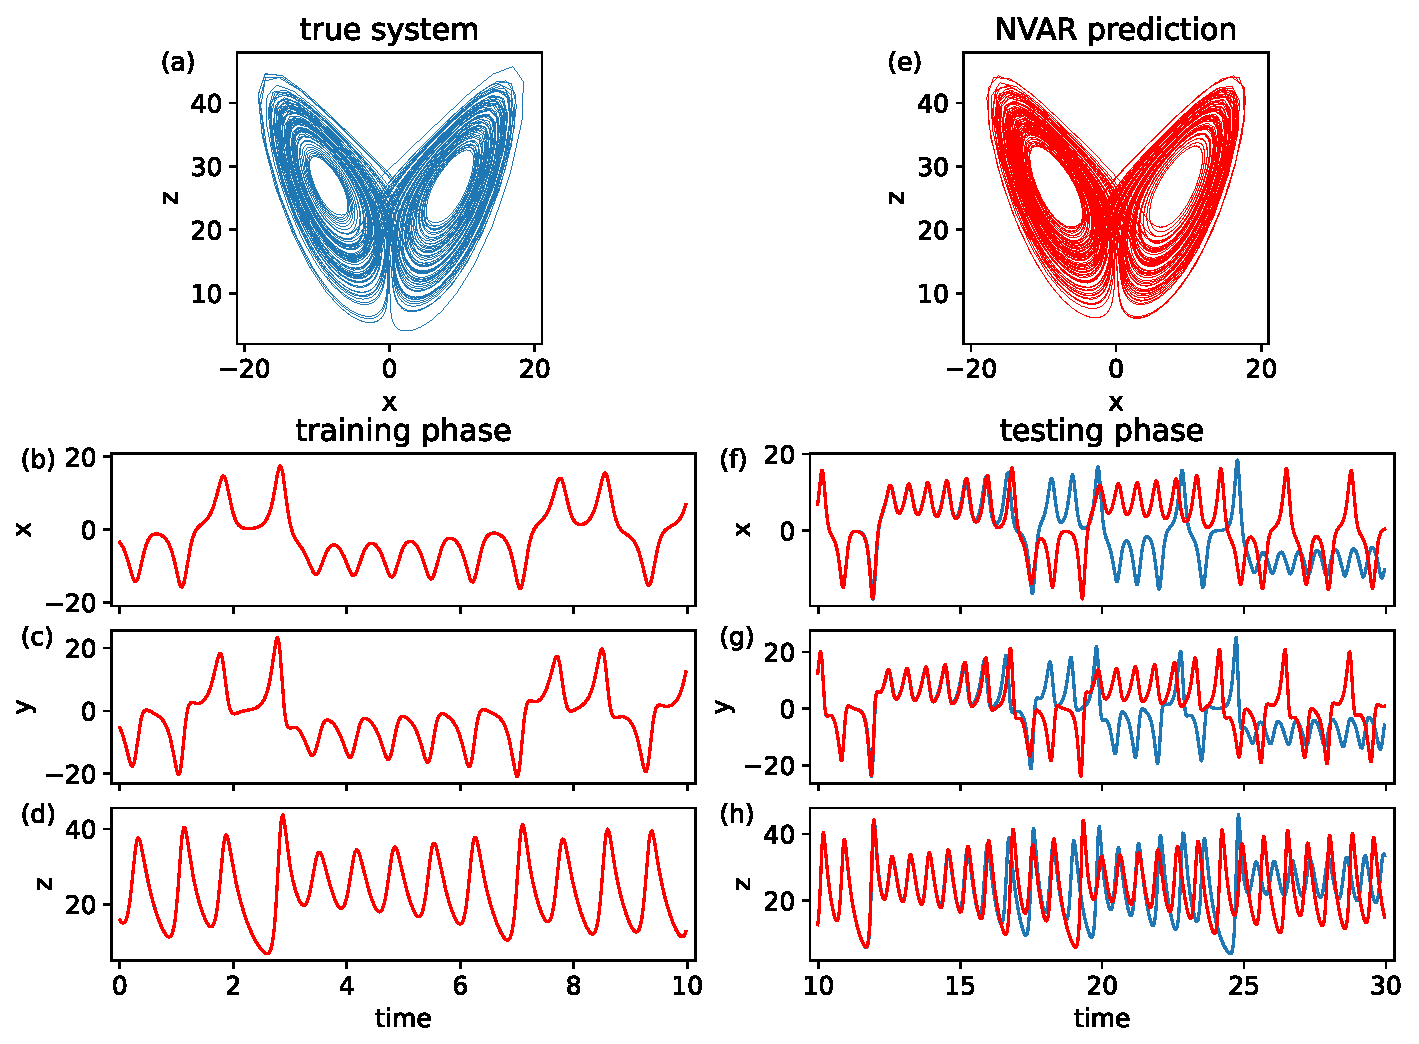
\includegraphics[width=0.9\textwidth]{figures/nvar-predict-lorenz}
  \end{center}
\end{frame}

% put rmap here if needed

\subsection{5.2.3 Output Weights}
\begin{frame}{Lorenz '63 Forecasting $W_\text{out}$}
  \begin{columns}
    \column{0.4\textwidth}
    \begin{itemize}
    \item Lorenz vector field is quadratic
    \item is NVAR only working because it has matching quadratic terms?
    \item \textbf{No.} Terms in Lorenz (in red) are not favored over others.
    \end{itemize}
    \column{0.6\textwidth}
    \centering
    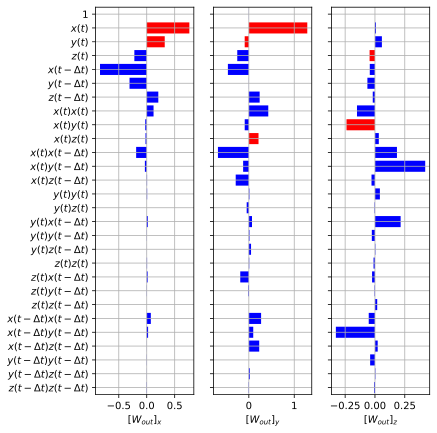
\includegraphics[width=1.0\textwidth]{figures/nvar-predict-lorenz-wout}
  \end{columns}
\end{frame}

%% \subsection{5.3 Forecasting the Double-Scroll Circuit}
%% \begin{frame}{Double-Scroll Forecasting}
%%   \begin{itemize}
%%   \item Goal: forecasting for double-scroll circuit
%%   \item two taps, $\tau_0 = 0$ and $\tau_1 = 1$
%%   \item $\Delta t = 0.25$ (40 points per Lyapunov period)
%%   \item $\bm{g}_\text{n}$ includes linear and cubic terms, to match symmetry
%%     $$ \bm{g}_\text{n}(\bm{v}) = \bm{v} \oplus \ceil{\bm{v} \otimes \bm{v} \otimes \bm{v}} $$
%%   \item train on 100 time units (400 data points)
%%   \item evaluate $\tilde{\epsilon}$ with 10 trials of $\epsilon_1$
%%   \end{itemize}
%% \end{frame}

%% \begin{frame}{Double-Scroll Forecasting Results}
%%   \begin{center}
%%     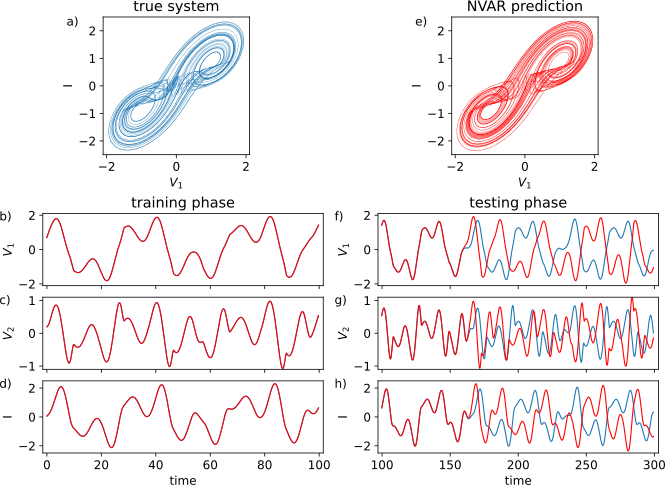
\includegraphics[width=0.8\textwidth]{figures/nvar-predict-dscroll}
%%   \end{center}
%%   \begin{itemize}
%%   \item NRMSE $\tilde{\epsilon} = 2.15\pm0.63\times10^{-2}$
%%   (~1.5$\times$ better)
%%   \end{itemize}
%% \end{frame}

%% \subsection{5.4 Forecasting Mackey-Glass}
%% \begin{frame}{Mackey-Glass Forecasting}
%%   \begin{itemize}
%%   \item Mackey-Glass system
%%     \begin{equation*}
%%       \dot{u}(t) = \beta \frac{u(t - 17)}{1 + u(t - 17)^{10}} - \gamma u(t),
%%     \end{equation*}
%%     with standard parameters $\beta = 0.2$, $\gamma = 0.1$.
%%     \vspace{2em}
%%   \item use three clusters of two taps each:
%%     \begin{itemize}
%%       \item $\tau_0 = 0$, $\tau_1 = 1$
%%       \item $\tau_2 = \floor{17/2\Delta t}$, $\tau_3 = \tau_2 + 1$
%%       \item $\tau_4 = \floor{17/\Delta t}$, $\tau_5 = \tau_4 + 1$
%%     \end{itemize}
%%   \item $\bm{g}_\text{n}$ includes constant up to cubic terms
%%     $$ \bm{g}_\text{n}(\bm{v}) = 1 \oplus \bm{v} \oplus \ceil{\bm{v} \otimes \bm{v}} \oplus \ceil{\bm{v} \otimes \bm{v} \otimes \bm{v}} $$
%%   \end{itemize}
%%   \blfootnote{\fullcite{mackey1977}}
%% \end{frame}

%% \begin{frame}{Mackey-Glass Forecasting Results}
%%   \begin{center}
%%     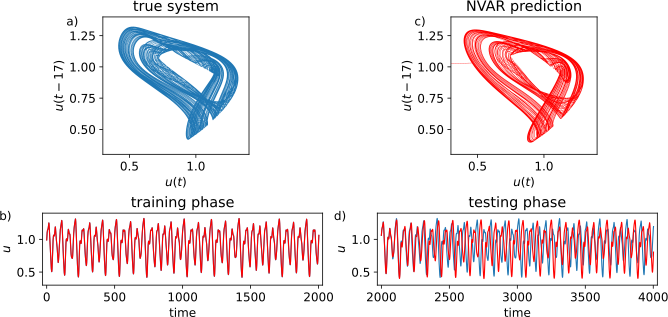
\includegraphics[width=0.9\textwidth]{figures/nvar-predict-mackey-glass}
%%   \end{center}
%%   \begin{itemize}
%%   \item NRMSE $\tilde{\epsilon} = 5.77\pm0.42\times10^{-2}$
%%   \end{itemize}
%% \end{frame}

\subsection{5.5 Conclusion}
\begin{frame}{Conclusion}
  Positives:
  \begin{itemize}
  \item NVARs have comparable performance to ESNs on Lorenz '63 and double-scroll circuit
  \item only need a few taps and low-order nonlinearity
  \item careful tap positioning can aid in keeping number of taps low
  \end{itemize}
  \vspace{1em}
  Possible improvements:
  \begin{itemize}
  \item $\bm{g}_\text{n}$ needs access to higher order terms without exponential explosion in size of $W_\text{out}$
  \item possible future research: using full nonlinear functions, rather than monomial terms
  \end{itemize}
\end{frame}

\section{Chapter 6: Conclusion}

\tocframe

\begin{frame}{Conclusion}
  \vspace{2em}
  Take-aways:
  \begin{itemize}
  \item ESNs are often more complicated than necessary
  \item NVARs are ESNs without any extra steps. Always try an NVAR first!
  \end{itemize}
  \vspace{1em}
  Topics for future research:
  \begin{itemize}
  \item any task previously done with an RC should be attempted with an NVAR -- both success and failure would be interesting!
  \item for ML, reframes VARs in a reservoir computing framework.
  \item for Physics, get a new simple ML approach that works well on physical problems
  \end{itemize}
\end{frame}

\begin{frame}
  \begin{center}
    {\usebeamercolor[fg]{frametitle}{\Large Thank you!}}

    Questions?
  \end{center}

  \note{o7}
\end{frame}

\end{document}

